%%%%%%%%%%%
%% Home work template for Graduate School
%% Author : Thamme Gowda N.
%% Originally from  https://github.com/thammegowda/hw-tex-templ
%%%%%%%%%%%%%%

\documentclass[letterpaper,doc,notimes]{apa6}
%%\documentclass[tikz]{standalone}
\usepackage{tikz}
%Required by APA6 package
\usepackage[normalem]{ulem}
\usepackage[english]{babel}
\usepackage[utf8x]{inputenc}
\usepackage{amsmath}
\usepackage{amssymb}
\usepackage{amsfonts}
\usepackage{graphicx}
\usepackage{adjustbox}

%Oft-used, oft-abused
\usepackage{afterpage}
\usepackage{booktabs}
\usepackage{caption}
\usepackage{censor}
\usepackage{color}
\usepackage{csquotes}
\usepackage{enumitem}
\usepackage{float}
\usepackage{hyperref}
\usepackage{lmodern}
%\usepackage{media9}
\usepackage{multirow}
\usepackage{outlines}
\usepackage{pdfpages}
\usepackage{placeins}
\usepackage{soul}
\usepackage{tabularx}
\usepackage[colorinlistoftodos]{todonotes}
\usepackage{xcolor}
\usepackage{mathtools}
\graphicspath{ {images/}}

\usepackage{sectsty}
\sectionfont{\fontsize{14}{12}\selectfont}

\setenumerate[1]{label=\Roman*.}
\setenumerate[2]{label=\Alph*.}
\setenumerate[3]{label=\roman*.}
\setenumerate[4]{label=\alph*.}

% break page where ever is required
\allowdisplaybreaks

\title{ \textbf{ USC CSCI 567 HOMEWORK 3 SOLUTIONS} }
\shorttitle{USC CSCI567 FALL16 HW3}
\author{\textsc{ThammeGowda Narayanaswamy}}
\affiliation{ tnarayan@usc.edu \\ ID : 2074-6694-39 \\ Department of Computer Science \\ Viterbi School of Engineering \\ University of Southern California \\ Los Angeles, CA 
	}


\note{\today}
%\note{ Collaborators : \\ Ishan Alok (ialok@usc.edu)}

\authornote{Produced for Fall 2016 session of CSCI 567, ``Machine Learning'', taught by Dr. Yan Liu at the University of Southern California}


\begin{document}

\maketitle
\newpage

\section{1.BIAS VARIANCE TRADE-OFF}
\subsection{a. Closed form Solution for Ridge Regression}
Given :
$$
\hat{\beta_\lambda} = argmin_\beta \bigg\{ \frac{1}{n} \sum_{i=1}{n}(y_i - x_i^T\beta)^2 + \lambda \parallel \beta \parallel_2^2 \bigg\}  \\
$$
In matrix form:
$$
\hat{\beta_\lambda} = argmin_\beta \bigg\{ \frac{1}{n} (Y - X\beta)^T (Y - X\beta) + \lambda  \beta^T \beta \bigg\}  \\
$$
where $X \in R^{n \times p}$ , $Y \in R^{n \times 1}$ and $\beta \in R^{p \times 1}$
We know that the above expression (assuming it is convex) is minimum  when its derivative is zero .
\begin{align*}
	\dfrac{\partial}{\partial\beta} \bigg[ \frac{1}{n} (Y - X\beta)^T (Y - X\beta) + \lambda  \beta^T \beta \bigg] = & 0 \\
\frac{1}{n} \dfrac{\partial}{\partial\beta} \bigg[ Y^TY - Y^T X\beta - (X\beta)^TY + (X\beta)^T(X\beta) +  \lambda  \beta^T \beta \bigg] = & 0 \\
 \dfrac{\partial}{\partial\beta} \bigg[ - Y^T X\beta - \beta^TX^TY + \beta^TX^TX\beta +  \lambda  \beta^T \beta \bigg] = & 0 \\
  - Y^T X -  X^TY + 2\beta^TX^TX +  2\lambda  \beta  = & 0 \\
				- 2 X^TY  + 2X^TX\beta +  2\lambda \beta  = & 0 \\
    [ X^TX +  \lambda I ] \beta  = &  X^T Y  \\
    \text{When $X^TX +  \lambda I$ is invertible, } & \\
     \beta  = & [ X^TX +  \lambda I ]^{-1}  X^T Y   \\
 \implies \hat{\beta_\lambda} = & [ X^TX +  \lambda I ]^{-1} X^T Y  \\
\end{align*}
We are told that the target label $y$ is from linear model plus an additional Gaussian noise $\epsilon$.\\
$\implies $ Distribution of $\epsilon$ is $N(0, \sigma^2)$\\
$\implies$ By applying affine transformations,  the distribution of $Y \approx N(X\beta^*, \sigma^2)$ \\
$\implies \text{Since  } \hat{\beta_\lambda} = H_\lambda Y \text{,  where} H_\lambda = [ X^TX +  \lambda I ]^{-1}  X^T$ \\
The distribution of $\hat{\beta_\lambda} \approx N (H_\lambda X \beta^*,   H_\lambda^T \sigma^2 I H_\lambda ) $ 

\subsection{b. Bias Term}
\begin{align*}
	bias = & \mathbb{E}[x^T\hat{\beta_\lambda}] - x^T\beta^* & \\
	      = &x^T[ \mathbb{E}[\hat{\beta_\lambda}] - \beta^*] &  \\
	      = & x^T[H_\lambda X \beta^* - \beta^*] & \because \text{from part a, the mean of Gaussian} \\
			 &where \text{ where} H_\lambda = [ X^TX +  \lambda I ]^{-1}  X^T & \\    
   bias = & x^T(H_\lambda X  - I) \beta^* & \\
\end{align*}
\subsection{c. Variance Term}
\begin{align*}
	variance = & \mathbb{E} \bigg[ \big( x^T\hat{\beta_\lambda} - \mathbb{E}[x^T\hat{\beta_\lambda}] \big)^2 \bigg] & \\
	= & \mathbb{E} \bigg[ \big( x^T (\hat{\beta_\lambda} - \mathbb{E}[\hat{\beta_\lambda}] )\big)^2 \bigg]  &\\
	= & \bigg( x^T ( \mathbb{E}\big[\hat{\beta_\lambda} - \mathbb{E}[\hat{\beta_\lambda}] \big] )\bigg)^2  &\\
	= &  x^T ( \mathbb{E}\big[\hat{\beta_\lambda} - \mathbb{E}[\hat{\beta_\lambda}] \big] )^2 x  &\\
  = & x^T  Var(\hat{\beta_\lambda})  x &\\
Variance  = & x^T  H_\lambda^T \sigma^2 I H_\lambda x &  \because From Part-a \\
    & \text{Where, } H_\lambda = [ X^TX +  \lambda I ]^{-1}  X^T
\end{align*}
 
\subsection{d. Impact of $\lambda$  on Squared Error}
From the bias-variance theorem we have, squared error is proportional to sum of $variance$ and $bias^2$ 

The impact of $\lambda$ on squared error is as follows:
\begin{itemize}
	\item When $\lambda$ is smaller, the bias is small but variance is high. Thus the model tight fits to seen samples with less generalization.
	\item When $\lambda$ is large, the bias is larger but variance is smaller. Thus the model under fits the samples with poor prediction.
	\item Thus we cannot have least bias and least variance at the same time, we need to settle for a trade off between these.
\end{itemize}
\section{2. KERNEL CONSTRUCTION}

\subsection{a. Positive linear combination of valid kernels is a valid kernel}
To prove: $k_3(x, x') = a_1k_1(x, x') + a_2k_2(x, x')$ is a valid kernel \\
Given: $k_1$ and $k_2$ are positive definite kernel functions. $a_1, a_2 \ge 0 $ \\
Proof:
    Since $k_1$ and $k_2$ are positive definite kernel functions, we have from Morcer theorem:
    \begin{equation}\label{eqn:1}
			\int_{x}\int_{x'}k_1(x, x') f(x) f(x') dx dx' \ge 0
    \end{equation}
    And 
    \begin{equation} \label{eqn:2}
   \int_{x}\int_{x'}k_2(x, x') f(x) f(x') dx dx' \ge 0
   \end{equation}
  $$
  \implies k_3(x, x') = a_1\int_{x}\int_{x'}k_1(x, x') f(x) f(x') dx dx' + a_2\int_{x}\int_{x'}k_2(x, x') f(x) f(x') dx dx' 
$$
From equations \ref{eqn:1},  \ref{eqn:2}, and $a_1 \ge 0 $, $a_2 \ge 0 $ \\
 $\implies$ R.H.S is $\ge 0$ \\
 $\implies k_3$ is a positive definite kernel function

\subsection{b. }
To prove: $k_4(x, x') = f(x) f(x')$ is a valid kernel \\
Given: $f(.)$ is an arbitrary real valued function\\
Proof: \\
Let $x$ and $x'$  $\in \mathbb{R}^{n}$ \\
We can represent $k_4(x,x')$ as matrix $K_4$, given by
$$ K_4= \begin{bmatrix}
f(x_1)f(x'_1) & f(x_1)f(x'_2) & ... & f(x_1)f(x'_n)  \\
... &  &  & ... \\
f(x_n)f(x'_1) & f(x_n)f(x'_2) & ... & f(x_n)f(x'_n)  \\
\end{bmatrix} $$
The matrix can be decomposed into product of two vectors $F^T$ and $F$ , $F$ $\in \mathbb{R}^n$, such that $K_4 = F^T. F $ where 

  $F =  \begin{bmatrix}  f(x_1)\\ f(x_2) \\ ... \\ f(x_n) \end{bmatrix} $ 

To prove that $k_4$ is a valid kernel, we have to prove that the matrix $K_4$ is positive definite.\\

Let us consider, $y \in \mathbb{R}^n$ \\
\begin{align*}
y^T K_4 y = & y^T F F^T y \\
    =& (F^T y) ^T F^T y \\
    =& \parallel F^T y \parallel_2^2
\end{align*}
Since $L_2$ norm is always positive, we can infer that for any  $y \in \mathbb{R}^n, y^T K_4 y \ge 0$

$\implies k_4 $ is a valid kernel by definition

\subsection{c. The product of valid Kernel is a valid kernel}
To prove: $k_5(x, x') = k_1(x, x') k_2(x, x')$ is a valid kernel\\
Given: $k_1$ and $k_2$ are positive definite kernel functions.\\
Proof: \\
Let us consider Kernel matrices $K_1$, $K_2$, and $K_5$ corresponding to $k_1$, $k_2$, and $k_5$.
By definition of kernel functions we can say that $K_1$ and $K_2$ are:
\begin{itemize}
	\item Symmetric
	\item Positive semi definite
\end{itemize}
We know that, product of two symmetric positive semi definite matrices is also symmetric positive semidefinite matrix. (necessary and sufficient for valid kernel )\\
$\implies$ Thus $k_5$ is a valid kernel.

\section{3. KERNEL REGRESSION}
\subsection{a. Optimal value of $w$}
Given: the cost function 
$$
	J(w) = \min_w \sum_n (y_i - w^Tx_i)^2 + \lambda \parallel w \parallel^2_2
$$
Where $\lambda \ge 0$ is regularization coefficient.\\
We know that, $J$ is minimal when $\frac{\partial J}{\partial w}$
 \begin{align*}
 \dfrac{\partial}{\partial w} \bigg[ \frac{1}{n} (y - Xw)^T (y - Xw) + \lambda  w^T w \bigg] = & 0 \\
 \dfrac{\partial}{\partial w} \bigg[ y^Ty - y^T Xw - (Xw)^Ty + (Xw)^T(Xw) +  \lambda  w^T w \bigg] = & 0 \\
 \dfrac{\partial}{\partial w} \bigg[ - y^T Xw - w^TX^Ty + w^TX^TXw +  \lambda  w^T w \bigg] = & 0 \\
 - y^T X -  X^Ty + 2w^TX^TX +  2\lambda w  = & 0 \\
 - 2 X^Ty  + 2X^TXw +  2\lambda w  = & 0 \\
 [ X^TX +  \lambda I ] w  = &  X^T y  \\
 \text{When $X^TX +  \lambda I_D$ is invertible, } & \\
 \implies w^* =  [ X^TX +  \lambda I_D ]^{-1} X^T y  & \\
 \end{align*}

\subsection{b. }
Given that $x_i \in \mathbb{R}^D$  has been transformed to $\phi_i(x) \in \mathbb{R}^T$ \\
Thus the input matrix is  $\Phi \in \mathbb{R}^{N\times T}$ .
Substituting the input matrix in the equation from part a, we get \\
\begin{equation}\label{eqn:3}
	w^* =  [ \Phi^T\Phi +  \lambda I_T ]^{-1} \Phi^T y 
\end{equation}
Let us consider the expression,
\begin{align*}
[ \Phi^T\Phi +  \lambda I_D ] \Phi^T  =& [ \Phi^T\Phi\Phi^T +  \lambda \Phi^T ] &  \because \text{Distributing} \Phi^T\\ 
[ \Phi^T\Phi +  \lambda I_D ] \Phi^T  =& \Phi^T[ \Phi\Phi^T +  \lambda I_N ]  &  \because \text{Moving to the left side} \Phi^T \\ 
 \Phi^T  =& [ \Phi^T\Phi +  \lambda I_D ]^{-1} \Phi^T[ \Phi\Phi^T +  \lambda I_N ]  & \because \text{Inverse Multiplied on left }\\ 
 \Phi^T[ \Phi\Phi^T +  \lambda I_N ]^{-1} =& [ \Phi^T\Phi +  \lambda I_D ]^{-1} \Phi^T   & \because \text{Inverse Multiplied on Right }\\ 
\end{align*}
Substituting the result in \ref{eqn:3}, we get \\
\begin{equation}\label{eqn:4}
w^* = \Phi^T[ \Phi\Phi^T +  \lambda I_N ]^{-1} y
\end{equation}
\subsection{c. }
Given a testing sample $\phi(x)$, the prediction is given by,\\
\begin{align*}
	\hat{y} =& w^{*T} \phi(x) & \\
				=&	(\Phi^T[ \Phi\Phi^T +  \lambda I_N ]^{-1} y)^T \phi(x) & \\
				=&	(y^T [ (\Phi\Phi^T +  \lambda I_N)^T ]^{-1} \Phi \phi(x) & \\
				=&	(y^T [(\Phi\Phi^T)^T +  \lambda I_N]^{-1} \Phi \phi(x) & \\				
\end{align*}
Lets define a matrix $K = \Phi\Phi^T \in \mathbb{R}^{N \times N}$, \\
and $k(x) = \Phi\phi(x) \in \mathbb{R}^T$ \\
Since $K$ is symmetric, $K^T = K$
$$ \therefore \hat{y} = (y^T [K+  \lambda I_N]^{-1} k(x)  $$

\subsection{d. }
When the dimension of feature transformation $\phi(x) \in \mathbb{R}^T, T$, is large, kernel regressions are computationally efficient than linear ridge regression.
$\because$ kernel regression computes the kernel matrix $K  $ which is $\mathbb{R}^{N\times N}$ without actually computing the transformations $\phi(x)$.
Without kernel trick, we have to compute $T \times T$ matrix which is an expensive operation when $T  \gg N$. 
\begin{itemize}
	\item \textbf{Learning}:
		\subitem Linear Ridge Regression: $O(T^3)$ time and $O(T^2)$ memory; $T$ is the dimension of new feature space.
		\subitem Kernel  Regression: $O(N^3)$ time and $O(N^2)$ memory; $N$ is the number of examples in training set.
	\item \textbf{Prediction}: 
		\subitem Linear Ridge Regression: $O(T)$ time, $T$ is the dimension of new feature space.
		\subitem Kernel Regression: $O(D)$ time, $D$ is the dimensions of original feature space
\end{itemize}

\section{4. SUPPORT VECTOR MACHINES}
\subsection{1. Linearly separable?}
No. They are not linearly separable (in 2d euclidean space).

\subsection{2.Maximum margin decision surface}
$$w = \begin{bmatrix}
	0 \\ 0 \\ 0 \\ 1
\end{bmatrix} $$
 \subsection{3.  Make it  non separable}
The data can be easily made non separable by adding a negative label at the same as a positive example (or vice versa). In practice, this issue is called training data contamination.
\begin{minipage}{0.3\textwidth}
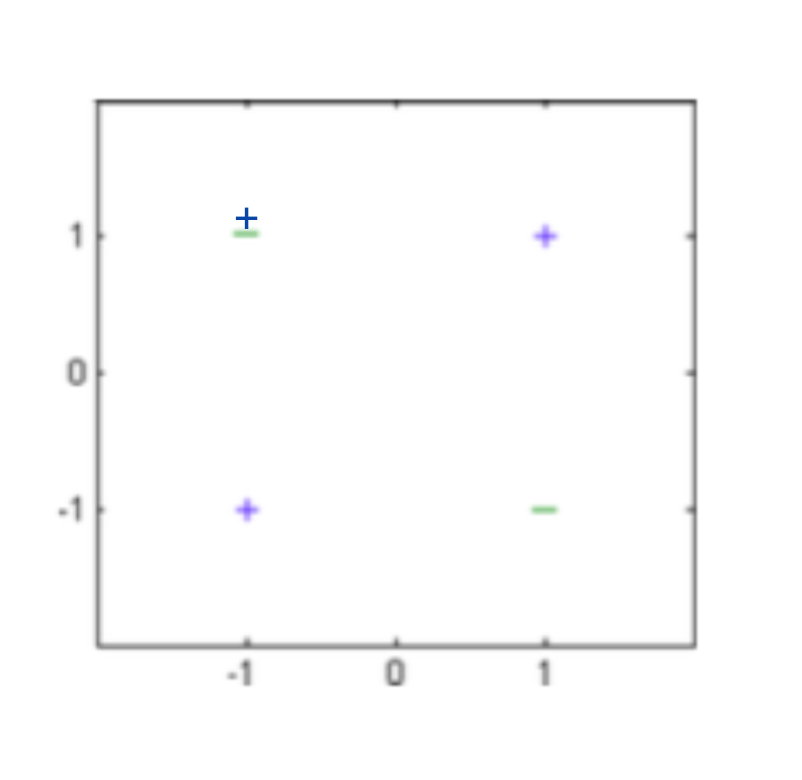
\includegraphics[scale=0.4]{4c}
\end{minipage}
\begin{minipage}{0.6\textwidth}\raggedleft
 Example: Adding positive example at (-1, 1)
\end{minipage}

\subsection{4. Kernel name}
\begin{align*}
	K(x,x) =& <\phi(x). \phi(x)>  = \phi(x)^T \phi(x) \\
	    =& [ \begin{smallmatrix}1 & x_1 & x_2 & x_1x_2  \end{smallmatrix} ]^T [ \begin{smallmatrix}1 & x_1 & x_2 & x_1x_2 \end{smallmatrix} ] \\
		=& 1 + x_1 + x_2 + x_1x_2   +   x_1 + x_1^2 + x_1x_2 + x_1^2x_2  +   x_2 + x_1x_2 + x_2^2 + x_1x_2^2  \\ 
		& + x_1x_2 + x_1^2x_2 + x_1x_2^2 + x_1^2x_2^2 
\end{align*}
This is a polynomial kernel.
\section{5. SVMs  AND THE SLACK PENALTY $C$}
\subsection{1. }
\begin{minipage}{0.5\textwidth} 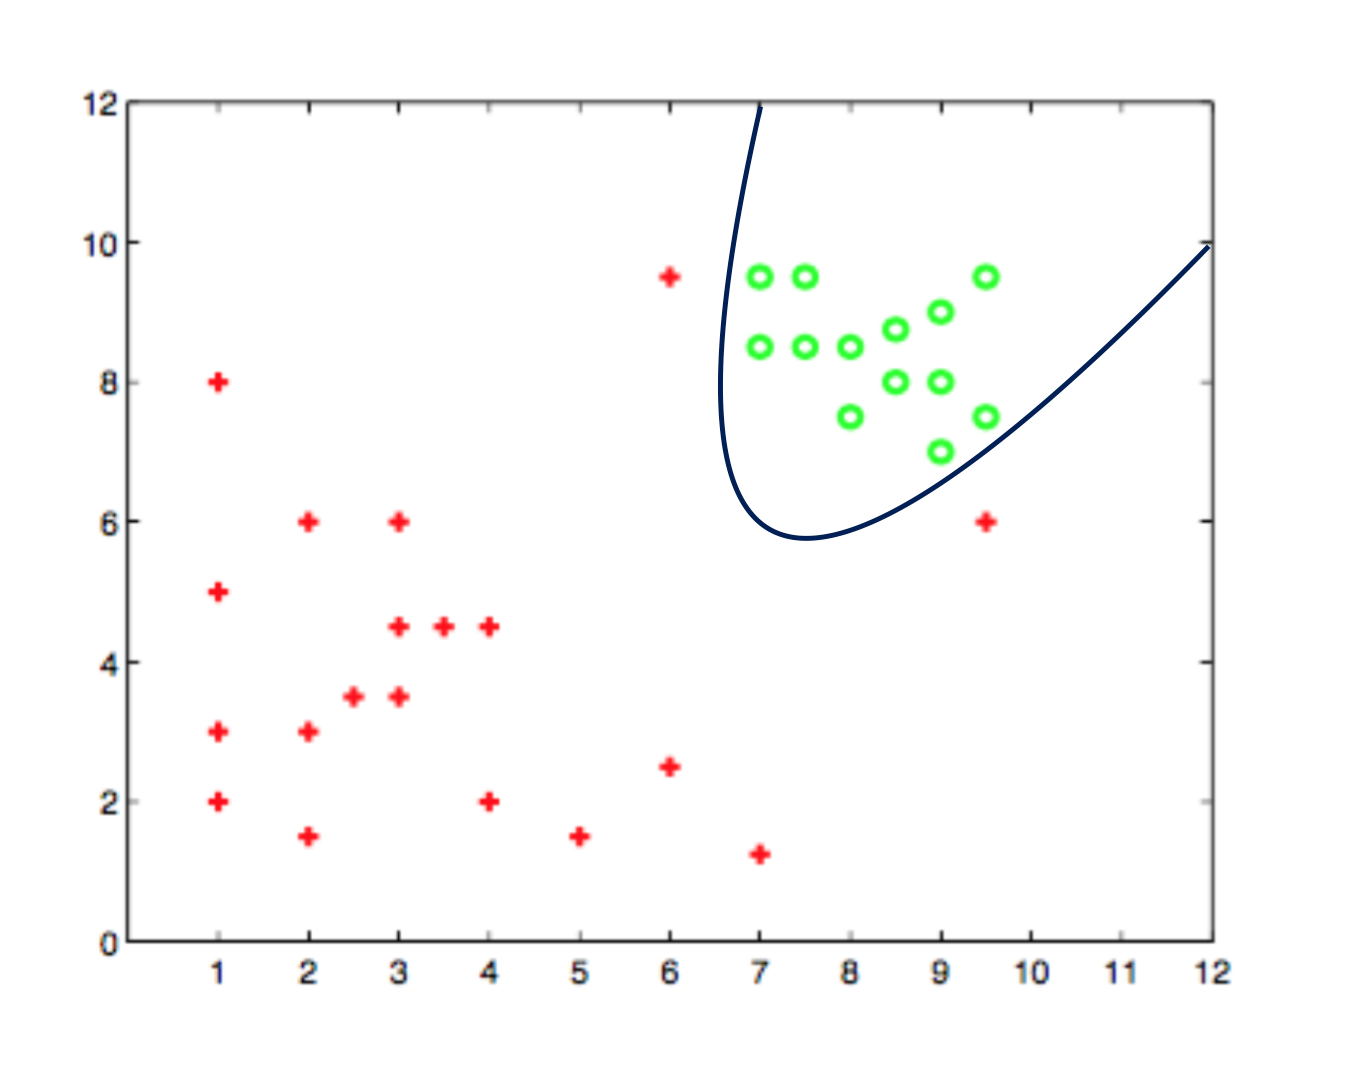
\includegraphics[scale=0.3]{5a} \end{minipage}
\begin{minipage}{0.5\textwidth}\raggedleft
When $C \rightarrow \inf$, SVM tends to minimize mis classification errors, even if the margin between the decision boundary plane and the training examples is small.
\end{minipage}
\subsection{2. }
\begin{minipage}{0.5\textwidth} 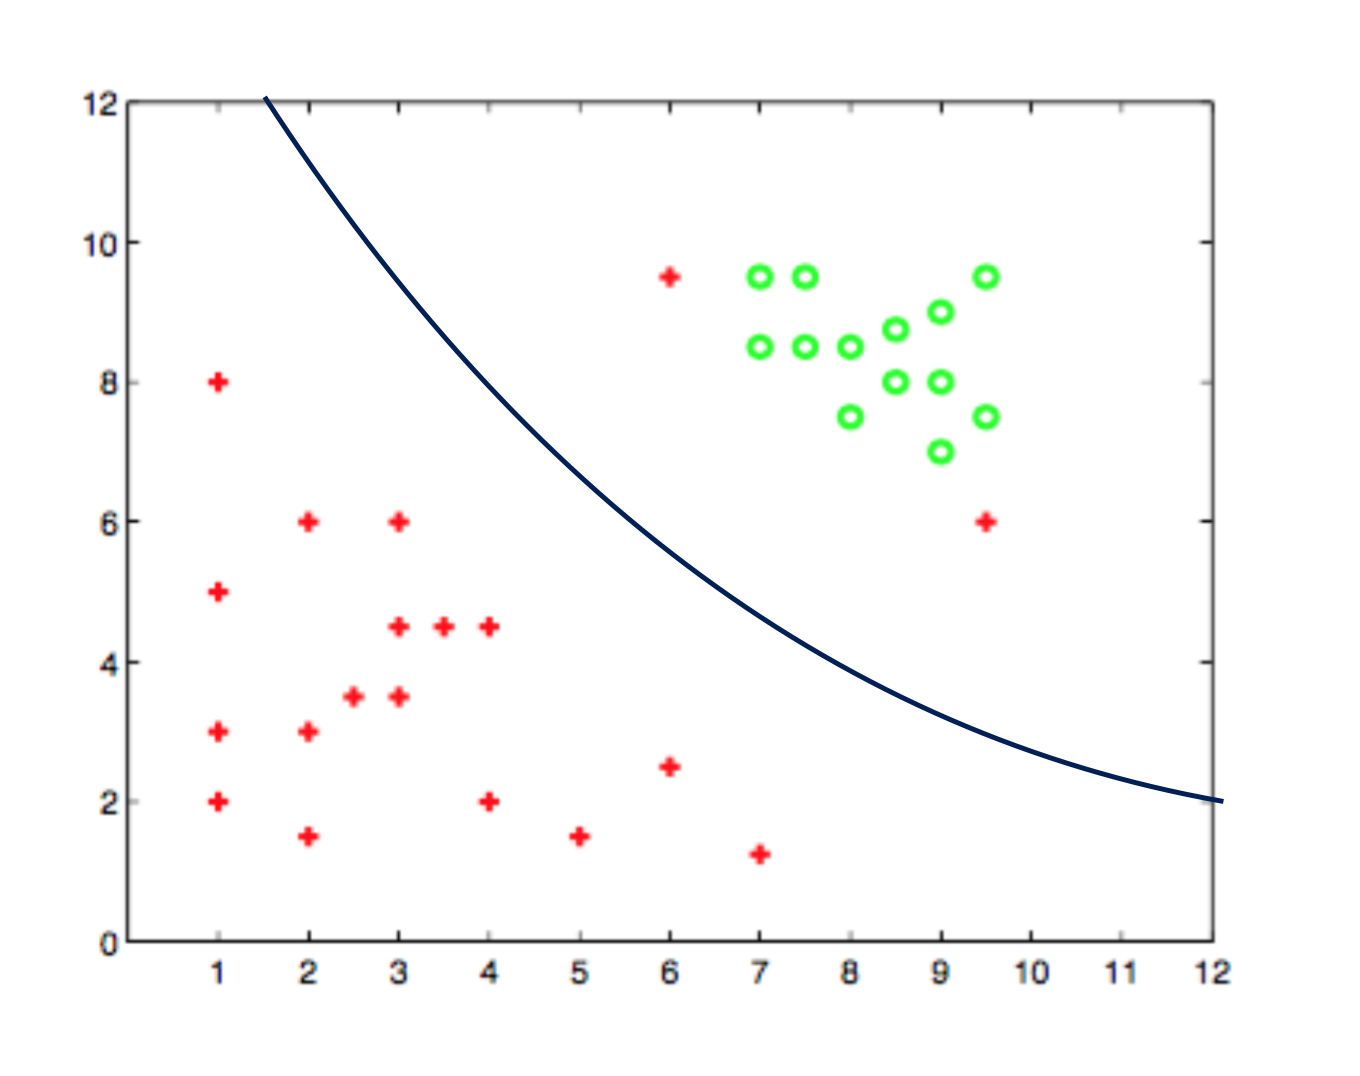
\includegraphics[scale=0.3]{5b} \end{minipage}
\begin{minipage}{0.5\textwidth}\raggedleft
	When $C \approx 0$, SVM tends to maximize the margin between the decision boundary and the training examples. This might even result in few mis classification errors.
 \end{minipage}
\subsection{3. }
The precision of Red Plus points and the Recall of the Green Circle points will be high.
Depending on the value of slack penalty (as discussed in the previous two sections), the recall of the Red Plus points and the precision of the Green circle points will vary and are most like to perform poorly. This is because there are few red plus points closer to green circle points which affect the position of the decision boundary.

\subsection{4. }
\begin{minipage}{0.5\textwidth} 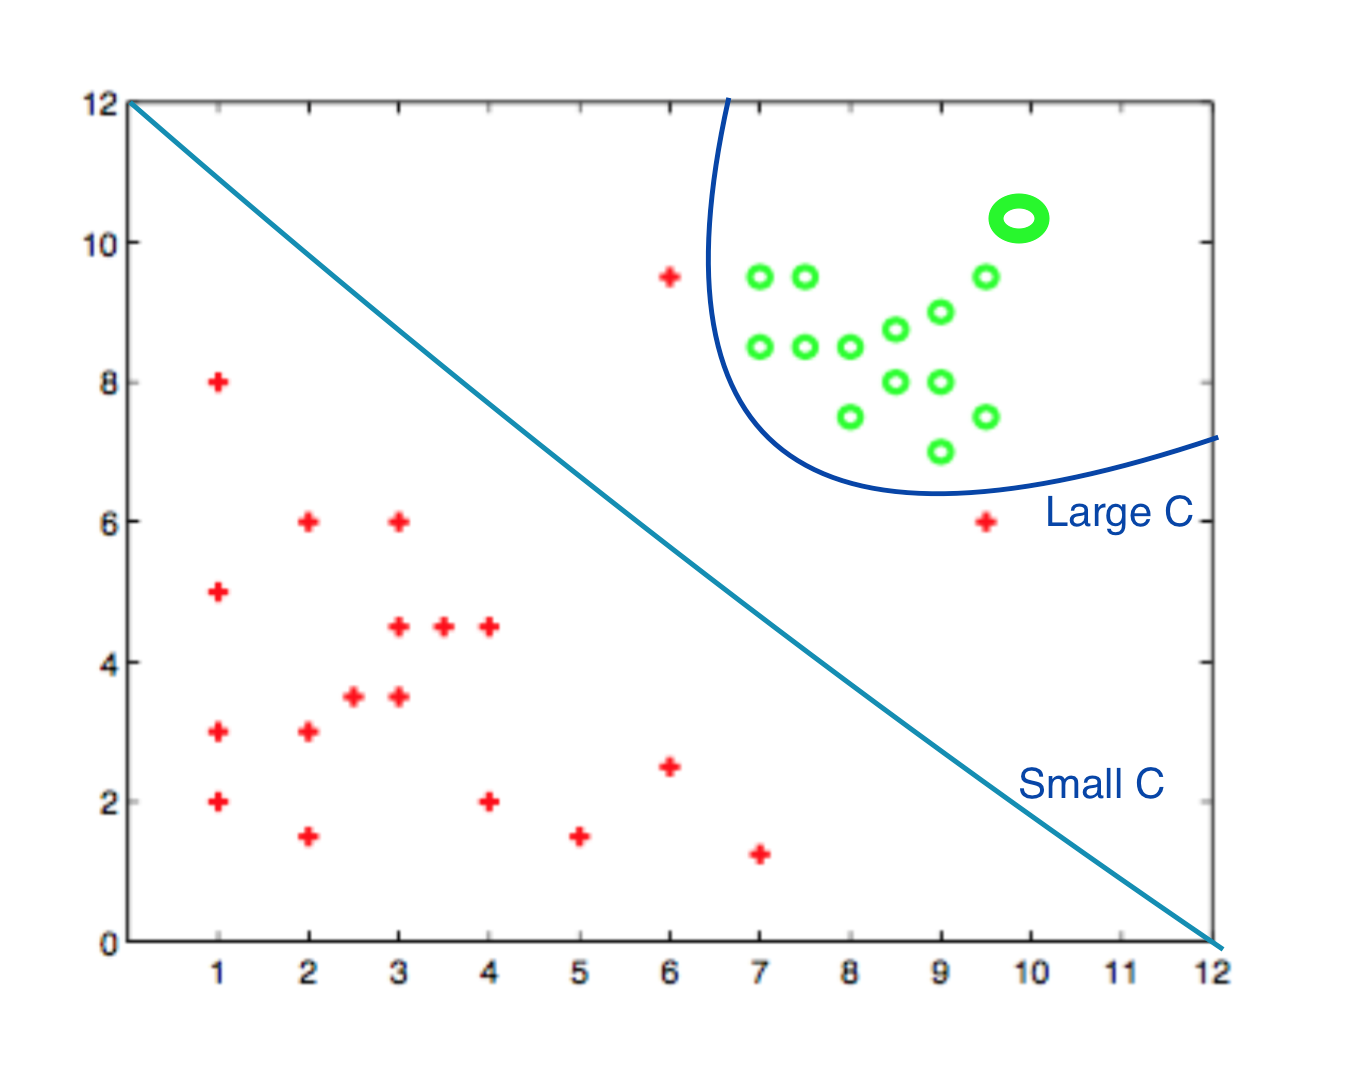
\includegraphics[scale=0.3]{5d} \end{minipage}
\begin{minipage}{0.5\textwidth}\raggedleft
	A point is added at the top right region of the plane. Since it is far from being a 'support vector', it doesnt change the decision boundary.
\end{minipage}

\subsection{5. }
\begin{minipage}{0.5\textwidth} 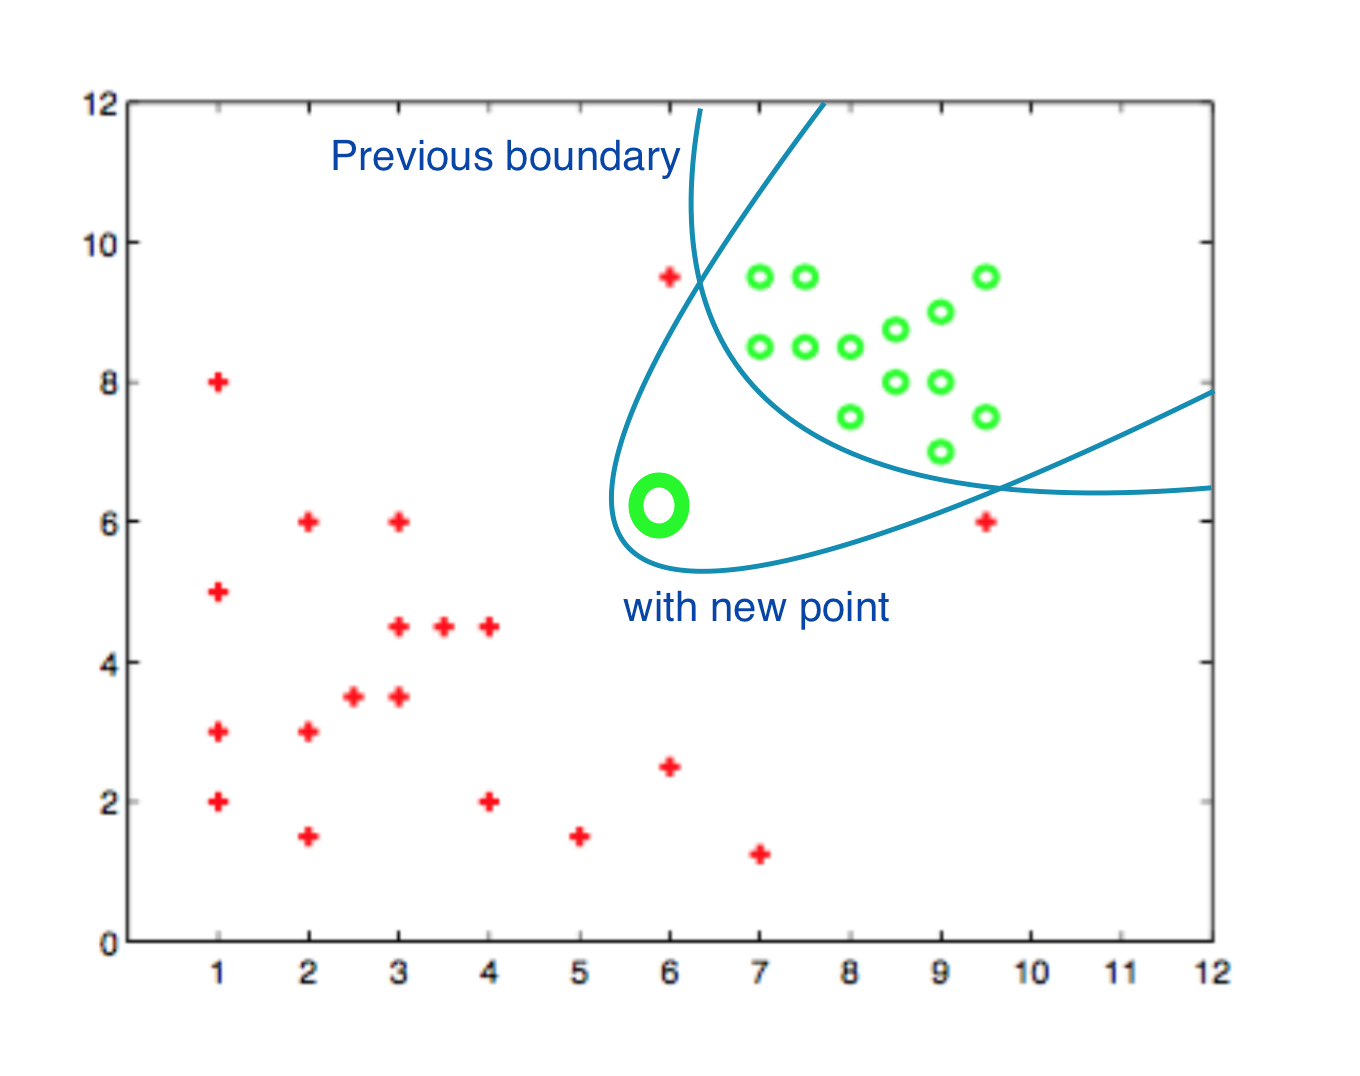
\includegraphics[scale=0.3]{5e} \end{minipage}
\begin{minipage}{0.5\textwidth}\raggedleft
	A point is added in between the decision boundary region. Since it becomes 'support vector', it participates in  forming the decision boundary.
\end{minipage}

\section{PROGRAMMING}
\subsection{Bias Variance}
\subsection{a. 10 samples per dataset}
Note:
  The evaluation is performed as follows based on the method suggested by TA's in one of the discussion sessions:
  \begin{itemize}
	\item Generated 100 datasets with 10 points each, $D_1, D_2, D_3... D_{100}$
	\item Built a model $h_{D_i}(.)$ for each 100 datasets.
	\item A news dataset $D_t$ is generated  for testing. 
	\item The bias and variance are measured based on the performance of 100 models on the $D_t$ dataset. 
  \end{itemize}
\subsection{Histograms}
The histograms are as follows \\
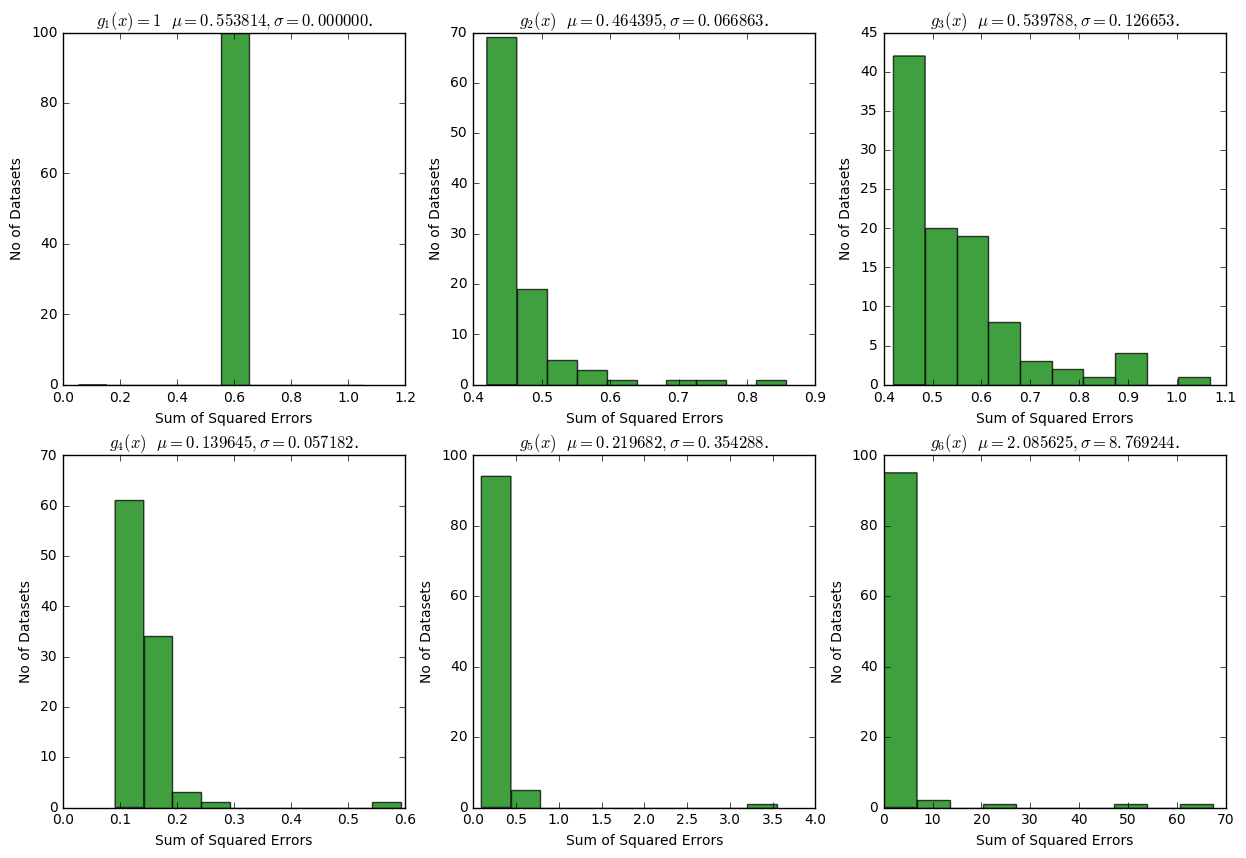
\includegraphics[width=1.0\textwidth]{hist_10samples}

The recorded $bias^2$ and variance are as follows:

\begin{tabular}{|c|c|c|} \hline
	Function & Variance      & $Bias^2$ \\ \hline
g1		& 0.00000000		& 0.55381366 \\
g2		& 0.04447961		& 0.41991505 \\
g3		& 0.11798539		& 0.42180300 \\
g4		 &0.04600876		& 0.09363664 \\
g5		 &0.12355812		& 0.09612371 \\
g6		 &1.98816964		& 0.09745515\\ \hline
\end{tabular}



\subsubsection{b. 100 Samples per dataset}
The histograms are as follows \\
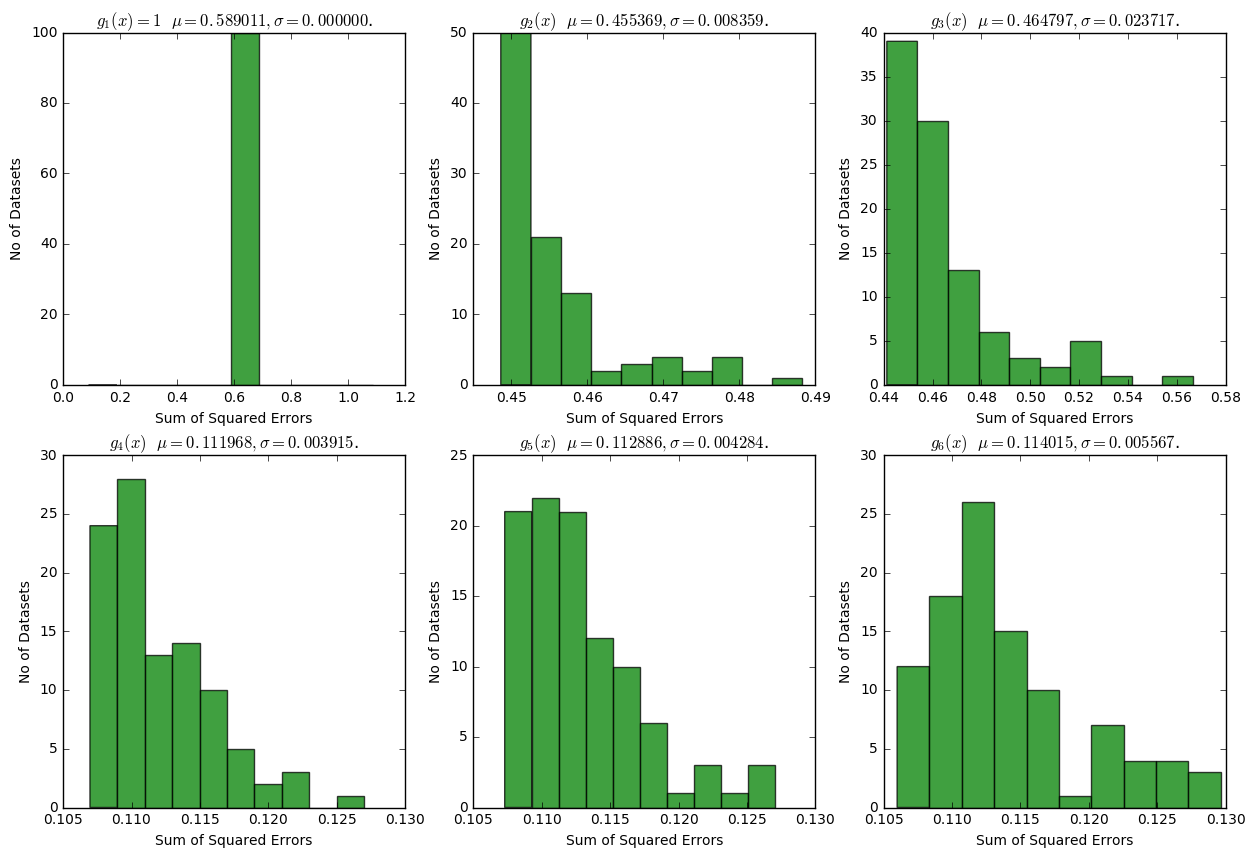
\includegraphics[width=1.0\textwidth]{hist_100samples}

The recorded $bias^2$ and variance are as follows:

 \begin{tabular}{|c|c|c|} \hline
	Function & Variance       & $Bias^2$ \\ \hline
g1		& 0.00000000		& 0.58901086 \\
g2		& 0.00464569		& 0.45072357 \\
g3		& 0.01270188		& 0.45209526 \\
g4		& 0.00269852		& 0.10926987 \\
g5		 &0.00366258		& 0.10922298 \\
g6		& 0.00511599		 & 0.10889857 \\ \hline
 \end{tabular}


\subsection{c. }
Key observations from this exercise:
\begin{itemize}
	\item As the model complexity increased, the bias decreased and the variance increased..
	\item When we added more number of samples to the dataset, we saw that the bias and variance continue to vary (bias decreased, variance increased) with increase in model complexity, however the magnitude of change is less. 
\end{itemize}

\subsection{d. Ridge Regression}
\begin{tabular}{|c|c|c|} \hline
Lambda	&  Variance	 &  $Bias^2$ \\ \hline
0.001	& 0.00291082	 & 0.110499 \\
0.003	& 0.00290983	& 0.110496 \\
0.01	& 0.00290636	 & 0.110483 \\
0.03	& 0.00289664	& 0.110451 \\
0.1	 & 0.00286453	 & 0.110368 \\
0.3	& 0.00278789	& 0.110376 \\
1	 & 0.00265098	& 0.11267 \\ \hline
\end{tabular}

Analysis: 
  As $\lambda$ increased, the bias increased and the variance decreased. 
  Thus $\lambda$ parameter can be used to control tight fitting by introducing the bias.
  
\subsection{Support Vector Machines}
\subsubsection{libSVM setup}
Using anaconda distribution:
\begin{verbatim}
	conda install -c conda-forge libsvm=3.21
\end{verbatim}
This installs two command line tools called \texttt{svm\_train} \texttt{svm\_predict}

\subsubsection{Using the Linear Kernel} 
The following results were recorded by using linear kernel type. 
The unit of average time is seconds for all the following results.
\begin{verbatim}
# LINEAR KERNEL
#             C  AvgTime   Accuracy%
1   0.000244141  0.213693  55.75
2   0.000976562  0.201526  55.75
3    0.00390625  0.197195  55.75
4      0.015625  0.190556  55.75
5        0.0625  0.196112  74.90
6          0.25  0.147726  92.05
7             1  0.100852  92.80
8             4  0.065552  95.10
9            16  0.053958  96.40
\end{verbatim}
Observation: The accuracy increased as we increased the slack penalty $C$, while the average training time decreased.

\subsubsection{Using the polynomial and RBF kernels} 
The following results were recorded:
\begin{verbatim}
# POLYNOMIAL KERNEL
#         C  Degree AvgTime   Accuracy%
1      0.015625  1  0.193540  55.75
2      0.015625  2  0.201199  55.75
3      0.015625  3  0.200625  55.75
4        0.0625  1  0.174386  90.35
5        0.0625  2  0.198155  89.00
6        0.0625  3  0.198131  74.90
7          0.25  1  0.103184  91.15
8          0.25  2  0.116746  92.15
9          0.25  3  0.147319  92.05
10             1  1  0.073813  92.85
11             1  2  0.079659  93.30
12             1  3  0.100888  92.80
13             4  1  0.056519  94.35
14             4  2  0.063589  94.90
15             4  3  0.067277  95.10
16            16  1  0.054508  94.30
17            16  2  0.057410  95.95
18            16  3  0.055024  96.40
19            64  1  0.056362  94.15
20            64  2  0.050879  96.65
21            64  3  0.051658  97.00
22           256  1  0.068880  94.50
23           256  2  0.053696  96.80
24           256  3  0.049736  96.90
25          1024  1  0.154141  94.50
26          1024  2  0.056765  96.50
27          1024  3  0.053674  96.55
28          4096  1  0.381076  94.50
29          4096  2  0.059383  96.75
30          4096  3  0.056649  96.60
31         16384  1  1.563308  94.70
32         16384  2  0.065256  96.45
33         16384  3  0.055341  96.60

# RBF KERNEL
#             C  Gamma    AvgTime    Accuracy%
1      0.015625  0.000061  0.196857  55.75
2      0.015625  0.000244  0.199696  55.75
3      0.015625  0.000977  0.193203  55.75
4      0.015625  0.003906  0.201737  55.75
5      0.015625  0.015625  0.200773  56.00
6      0.015625  0.062500  0.198204  87.30
7      0.015625  0.250000  0.200537  60.30
8        0.0625  0.000061  0.199040  55.75
9        0.0625  0.000244  0.200937  55.75
10        0.0625  0.000977  0.196819  55.75
11        0.0625  0.003906  0.203154  64.40
12        0.0625  0.015625  0.165145  90.55
13        0.0625  0.062500  0.128067  92.20
14        0.0625  0.250000  0.172642  92.05
15          0.25  0.000061  0.200721  55.75
16          0.25  0.000244  0.199568  55.75
17          0.25  0.000977  0.199016  66.60
18          0.25  0.003906  0.154790  90.85
19          0.25  0.015625  0.103935  91.40
20          0.25  0.062500  0.082446  93.10
21          0.25  0.250000  0.115713  95.55
22             1  0.000061  0.196611  55.75
23             1  0.000244  0.198686  67.85
24             1  0.000977  0.152969  91.05
25             1  0.003906  0.099703  91.40
26             1  0.015625  0.074173  93.50
27             1  0.062500  0.063382  95.90
28             1  0.250000  0.085199  97.15
29             4  0.000061  0.197674  67.95
30             4  0.000244  0.151894  90.85
31             4  0.000977  0.102306  91.45
32             4  0.003906  0.072589  93.35
33             4  0.015625  0.056027  94.90
34             4  0.062500  0.054397  96.80
35             4  0.250000  0.074961  96.95
36            16  0.000061  0.154246  90.85
37            16  0.000244  0.097384  91.50
38            16  0.000977  0.074993  93.45
39            16  0.003906  0.057111  94.55
40            16  0.015625  0.053216  95.85
41            16  0.062500  0.052186  97.10
42            16  0.250000  0.075502  96.70
43            64  0.000061  0.097574  91.50
44            64  0.000244  0.069576  93.45
45            64  0.000977  0.058329  94.45
46            64  0.003906  0.056718  94.50
47            64  0.015625  0.054045  96.75
48            64  0.062500  0.049619  97.00
49            64  0.250000  0.074851  96.70
50           256  0.000061  0.071727  93.45
51           256  0.000244  0.058747  94.40
52           256  0.000977  0.056307  94.30
53           256  0.003906  0.055413  95.90
54           256  0.015625  0.054942  97.20
55           256  0.062500  0.047539  96.85
56           256  0.250000  0.074552  96.70
57          1024  0.000061  0.057464  94.40
58          1024  0.000244  0.057587  94.40
59          1024  0.000977  0.056671  94.60
60          1024  0.003906  0.066289  96.70
61          1024  0.015625  0.057694  96.90
62          1024  0.062500  0.049985  96.85
63          1024  0.250000  0.076784  96.70
64          4096  0.000061  0.055695  94.40
65          4096  0.000244  0.058861  94.35
66          4096  0.000977  0.073948  96.20
67          4096  0.003906  0.086435  97.10
68          4096  0.015625  0.065810  96.95
69          4096  0.062500  0.050349  96.85
70          4096  0.250000  0.074639  96.70
71         16384  0.000061  0.060005  94.25
72         16384  0.000244  0.080497  94.70
73         16384  0.000977  0.114950  96.55
74         16384  0.003906  0.110726  96.75
75         16384  0.015625  0.065220  96.95
76         16384  0.062500  0.048876  96.85
77         16384  0.250000  0.073846  96.70

\end{verbatim}

Observation :
The best cross validation accuracy is $97.20\% $ and the corresponding parameters are $Kernel= RBF; C=256; gamma=0.015625$

The model built from these parameters recorded $98.5\%$ accuracy on the test dataset.

\end{document}